% ======================================================================
%\subsection{Rigorous upper bounds}

%----------------------------------------------------------------------
% \begin{frame}[shrink]%[allowframebreaks]
%   \frametitle{ Rigorous upper bounds}

%   \begin{itemize}
%   \item
%     Nicolaenko, Scheurer and Temam\rf{NSTks85}
%     $
%     \limsup_{t\to\infty}\norm{u}_2 = O(L^{\frac{5}{2}})
%     \,.
%     $
%     in the antisymmetric subspace.

%   \item
%     This antisymmetric assumption was removed by
%     Goodman\rf{Good94}.

%   \item
%     Collet \etal\rf{CEEksgl93} improved the result:
%     \[
%       \limsup_{t\to\infty}\norm{u}_2 = O(L^{\frac{8}{5}})
%       \,.
%     \]

%   \item
%     Bronski and Gammbill\rf{bronski2005}:
%     $\limsup_{t\to\infty}\norm{u}_2 = O(L^{\frac{3}{2}})$.

%   \item
%     Giacomelli and Otto\rf{GiacoOtto05}:
%     $ \limsup_{t\to\infty}|\!|u|\!|_2 = o(L^{\frac{3}{2}})$.


%   \item Otto\rf{Otto09} shows that
%     \[
%       \limsup_{t\to\infty} \frac{1}{T}\int_0^T dt \norm{|\partial_x|^\alpha u}^2
%       = O(L\cdot\ln^{10/3} L)
%       \,,\qquad 1/3 < \alpha \le 2
%       \,.
%     \]
%   \end{itemize}

%   \pause

%   Bronski and Gammbill\rf{bronski2005}
%   claim that $1/2$ is believed to be the best possible exponent.

% \end{frame}

% ======================================================================
\subsection{Estimate the dimension of the inertial manifold by \Fv s}

% ----------------------------------------------------------------------
\begin{frame}[shrink]%[allowframebreaks]
  \frametitle{Decoupling of local Floquet exponents}

  {\centering
    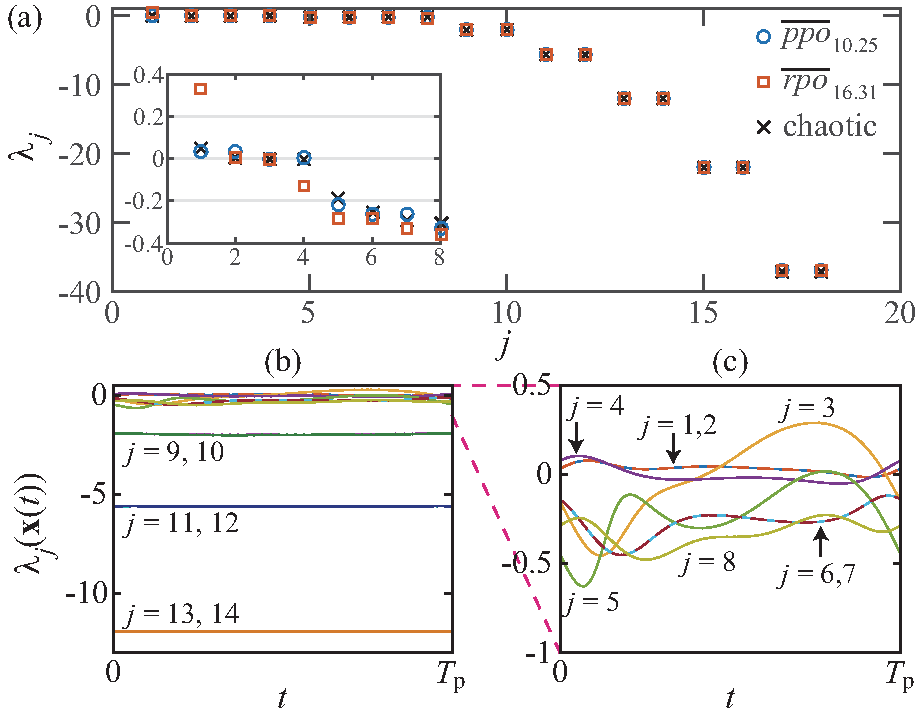
\includegraphics[width=0.8\textwidth]{ks22FloqExp}
    \par}
  

\end{frame}

% ----------------------------------------------------------------------
\begin{frame}[shrink]%[allowframebreaks]
  \frametitle{Decoupling of \Fv s}

  {\centering
    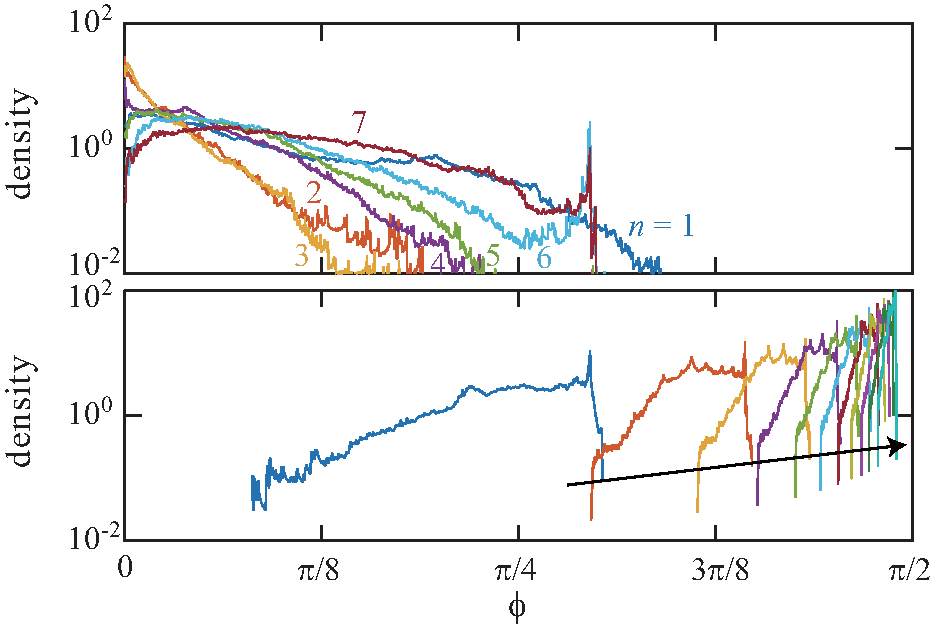
\includegraphics[width=0.9\textwidth]{ks22vecAngles}
  \par}

\end{frame}

% ----------------------------------------------------------------------
\begin{frame}[shrink]%[allowframebreaks]
  \frametitle{Shadowing controlled by \Fv s}

  {\centering
    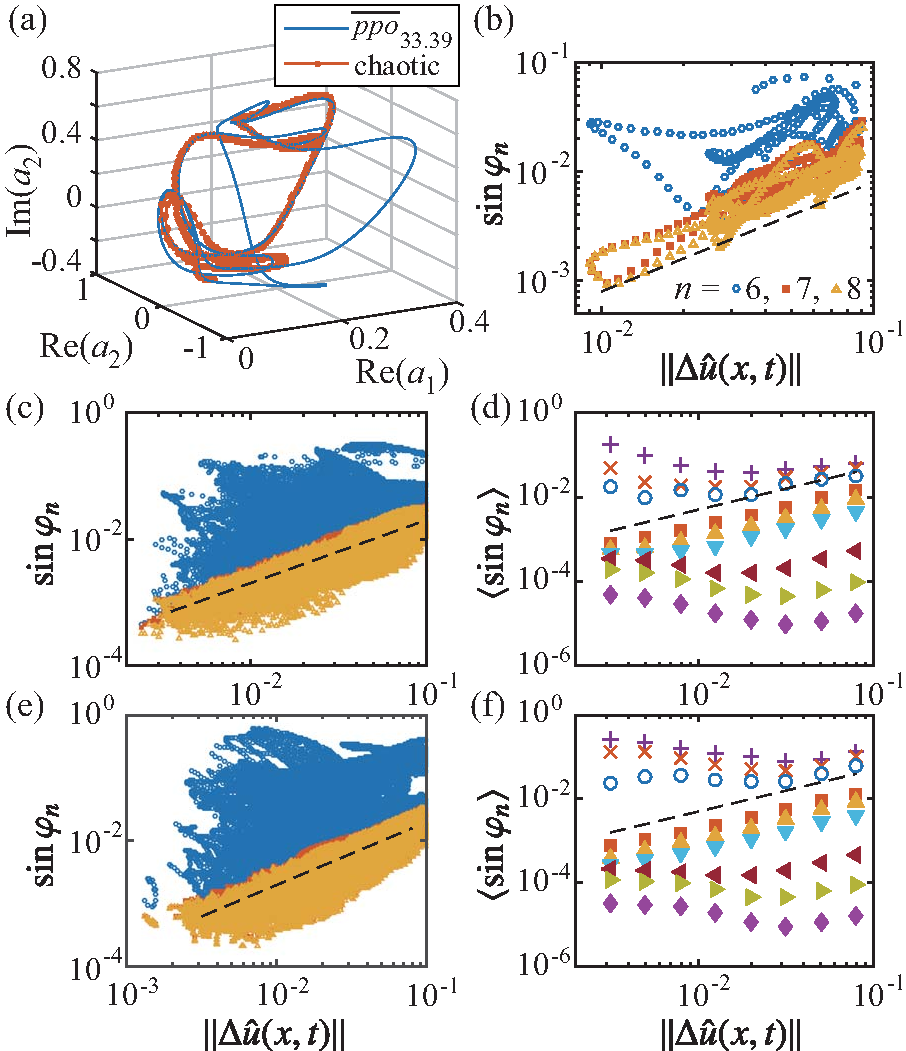
\includegraphics[width=0.6\textwidth]{ks22vecShadow}
    \par}

\end{frame}

% ----------------------------------------------------------------------
\begin{frame}%[allowframebreaks]
  \frametitle{Main result}

  \htbc{
    (Our simulations use 62 degrees of freedom.)
  }

  \vfill
  
  \htrc{
    For one-dimensional Kuramoto-Sivashinsky equation defined on a periodic
    domain of size L = 22, the dimension of the inertial manifold is 8.
  }

  \vfill 
  
  \setbeamercolor{block title}{fg=white, bg=green!75!black}
  \begin{block}{}
    \textrm{
      \small
      Ding, X., Chat\'e, H., Cvitanovi\'c, P., Siminos, E., and Takeuchi, K. A.,
      ``Estimating the dimension of the inertial manifold from unstable
      periodic orbits,''
      {\color{red}\emph{ Phys. Rev. Lett.}} {\bf 117}, 024101 (2016)
    }
  \end{block}
\end{frame}
